	\section{Domain}
		Nachfolgend werden die wichtigsten Bezeichnungen von Domänenobjekten eingeführt:
		
		\begin{description}
			\item[Problem] Beschreibt eine Vorlage für ein Designproblem eines Software Projektes, 
				z.B. ``Session State''. 
				Im Decision Knowledge System werden Problems als ``Problem Template'' bezeichnet.
			\item[Alternative] Beschreibt eine Vorlage für eine Wahlmöglichkeit eines Problems.
				Für das Problem ``Session State'' wären dies z.B. ``Server Session State'' und
				``Database Session State''. 
				Im Decision Knowledge System werden Alternatives als ``Option Template'' bezeichnet.
			\item[Decision] Beschreibt eine konkrete Problem Instanz.
				Decisions entstehen, wenn Problems auf konkrete Projekte angewendet werden.
				Decisions sind sowohl geschlossene wie noch zu treffende Entscheidungen.
				Im Decision Knowledge System werden Decisions als ``Problem Occurences'' bezeichnet.
			\item[Option] Beschreibt eine Wahlmöglichkeit einer Decisions, 
				und somit eine konkrete Instanz einer Alternative.
				Im Decision Knowledge System werden Options als ``Option Occurences'' bezeichnet.
			\item[Tasktemplate] Beschreibt eine Vorlage zum Erstellen von konkreten Tasks.
				Task Templates enthalten generische Werte, wie z.B. ``Project Manager'' als
				Attributwert für die Eigenschaft ``Assignee''.
			\item[Task] Beschreibt einen aus einem Tasktemplate erzeugten konkreten Task.
				Task entstehen während dem Übertragen der Informationen eines Tasktemplates an ein Projektplanungstool.
			\item[Mapping oder DKS Mapping] Bezeichnet die Verknüpfung von Problems oder 
				Alternatives mit einem Tasktemplate. 
				Anhand dieser Verknüpfung werden aus den verknüpften Tasktemplates und den Decisions oder Options des verknüpften Problem oder
				der verknüpften Alternative die Informationen generiert, 
				die für die Übertragung eines Tasks an ein Projektplanungstool benötigt werden.
			\item[Requesttemplate] Bezeichnet eine Vorlage für einen HTTP-Request um 
				in einem spezifischen Projektplanungstool Tasks anzulegen.
				Requesttemplates beinhalten Platzhalter (Variablen und Funktionen, sog. Processors),
				die mit Daten der Tasktemplates und Decisions oder Options ersetzt werden. 
		\end{description}	
	
	
		\subsection{Domainmodel}
			Die \eeppi\ Domain setzt sich aus drei Typen von Domänen Objekten zusammen: 
			\begin{itemize}
				\item Einer Abstraktion der Objekte hinter der Schnittstelle der angebundenen Entscheidungswissensverwaltung
				\item Einer Abstraktion der Objekte hinter der Schnittstelle eines oder mehreren angebundenen Projektplanungstools
				\item Den eigenen Objekten und Schnittstellen
			\end{itemize}
			
			Innerhalb von \eeppi\ werden nur die eigenen Objekte persistiert.
			Die Objekte der andern System werden On-Demand über die Schnittstellen geladen.
		
			\begin{landscape}
				\begin{figure}[H]
					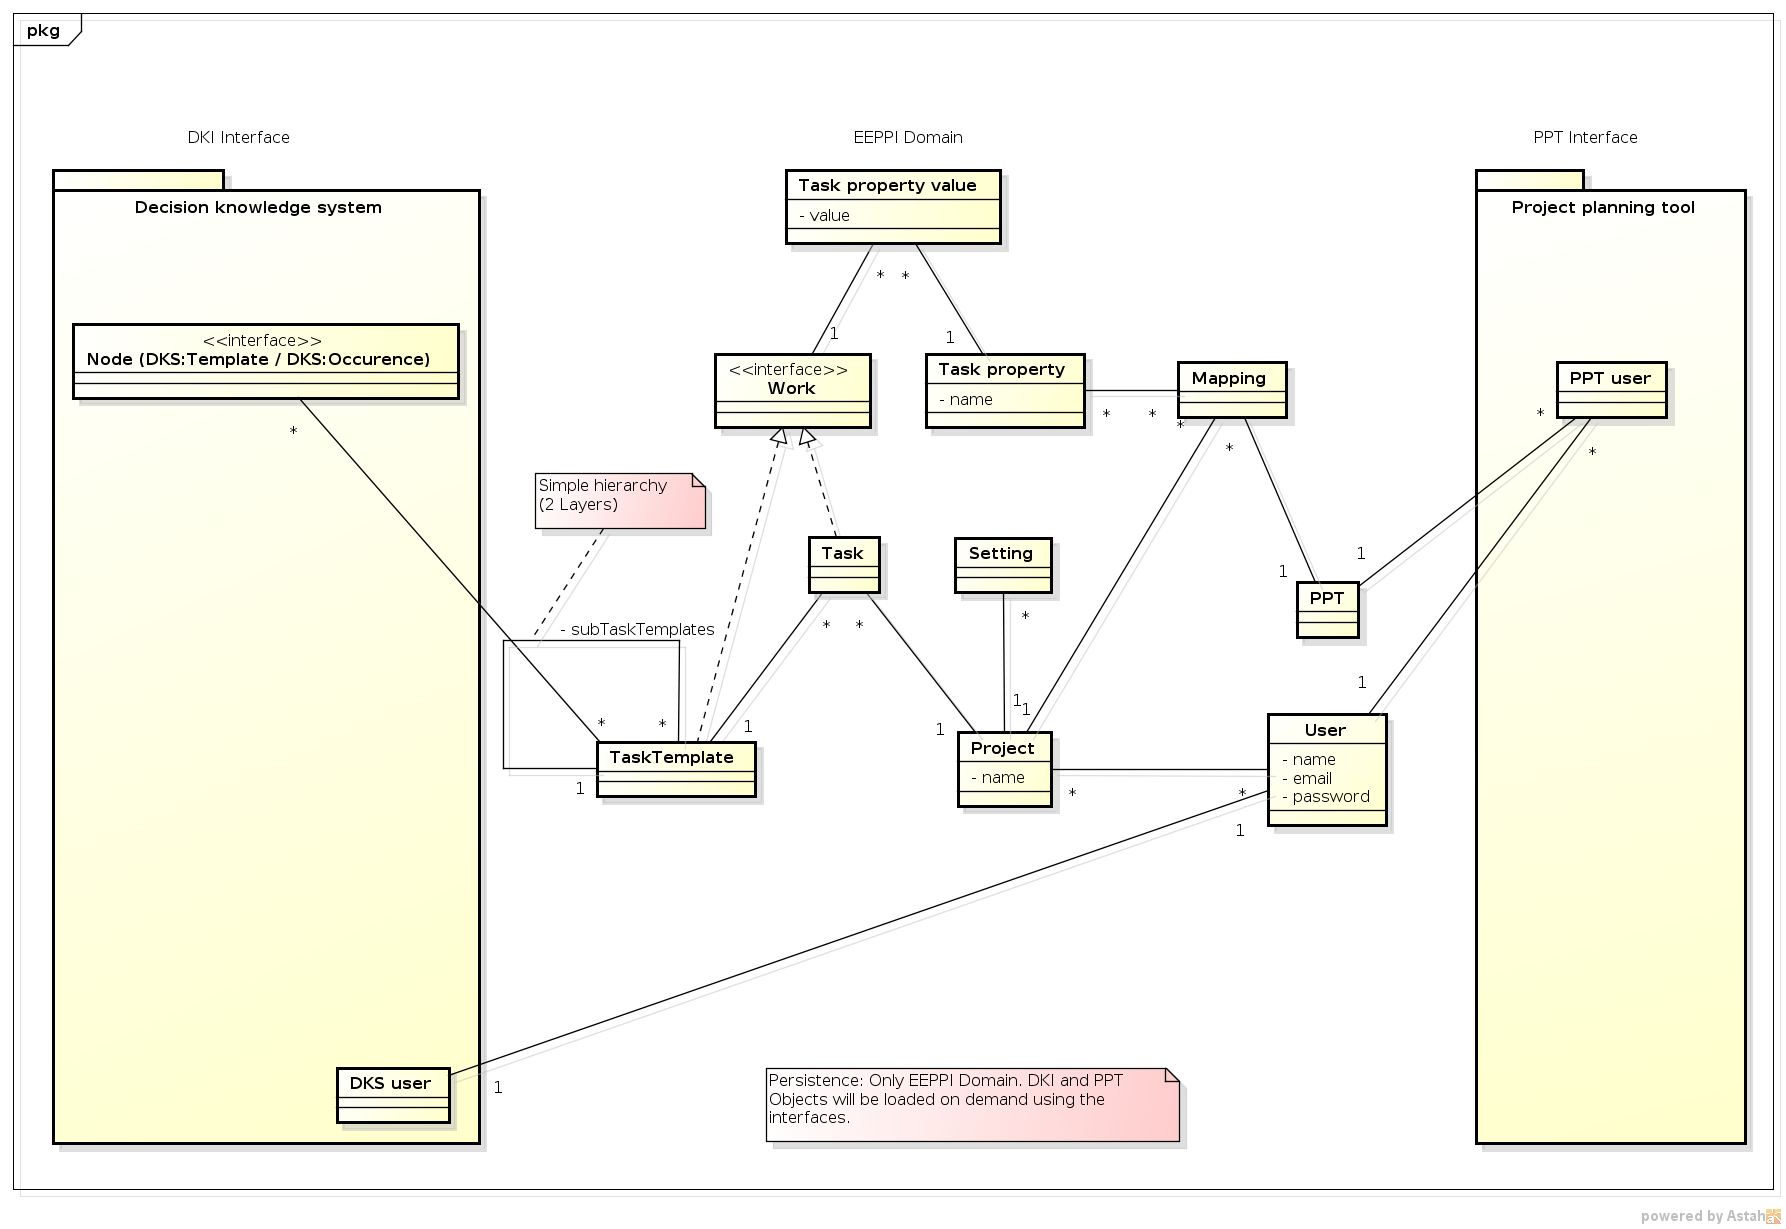
\includegraphics[width=0.9\linewidth]{architecture/media/img/domain.png}
					\centering
					\caption{\eeppi Domain}
					\label{fig:domain}
				\end{figure}				
			\end{landscape}
			
			\eeppi\ arbeitet mit den Objekten des DKS. Das DKS ist wie folgt aufgebaut:
			\begin{figure}[H]
				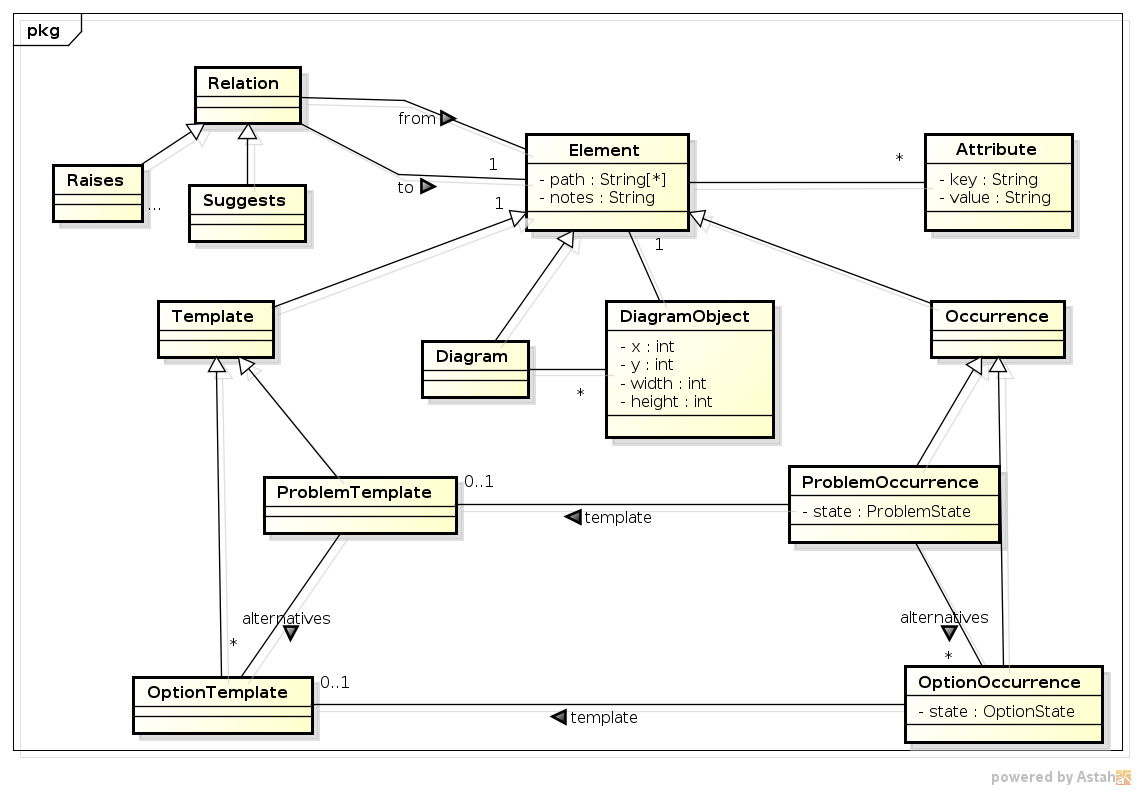
\includegraphics[width=\linewidth]{architecture/media/img/dksDomain.png}
				\centering
				\caption[DKS Domain\newline 
					\license{Eclipse Public License \url{https://www.eclipse.org/legal/epl-v10.html} Lukas Wegmann, IFS HSR \url{https://www.ifs.hsr.ch}}
				]{DKS Domain}
				\label{fig:dksDomain}
			\end{figure}
			
			Dabei werden die DKS Objekte wie folgt gemappt:
			\begin{description}
				\item[Element] Node
				\item[ProblemTemplate] Problem
				\item[ProblemOccurance] Decision			
			\end{description}						
			
			
		\subsection{Umbenennen und Löschen von Domänenobjekten}
			Um Probleme mit referenzierten Domänenobjekten zu vermeiden,
			darf es Benutzern nur möglich sein, Task Vorlagen umzubenennen,
			nicht jedoch zu löschen.
			Dies ermöglich Benutzern, 
			falsch angelegte Task Vorlagen weiterzuverwenden, vermeidet jedoch, 
			das bereits referenzierte Vorlagen entfernt werden.
			
			Das Gleiche gilt auch für Task Properties.
			Dies dürfen auf keinen Fall vom Benutzer entfernt werden 
			und dürfen entsprechend nur umbenannt werden.
			
		
		\subsection{Task-Vorlagen Strukturierung}
			Es gibt verschiedene Möglichkeiten, 
			Benutzer eine Strukturierung von Task-Vorlagen anzubieten.
			Task-Templates können selbst in eine Struktur gebracht werden, 
			oder durch externe Strukturen geordnet werden.
		
			\begin{figure}[H]
				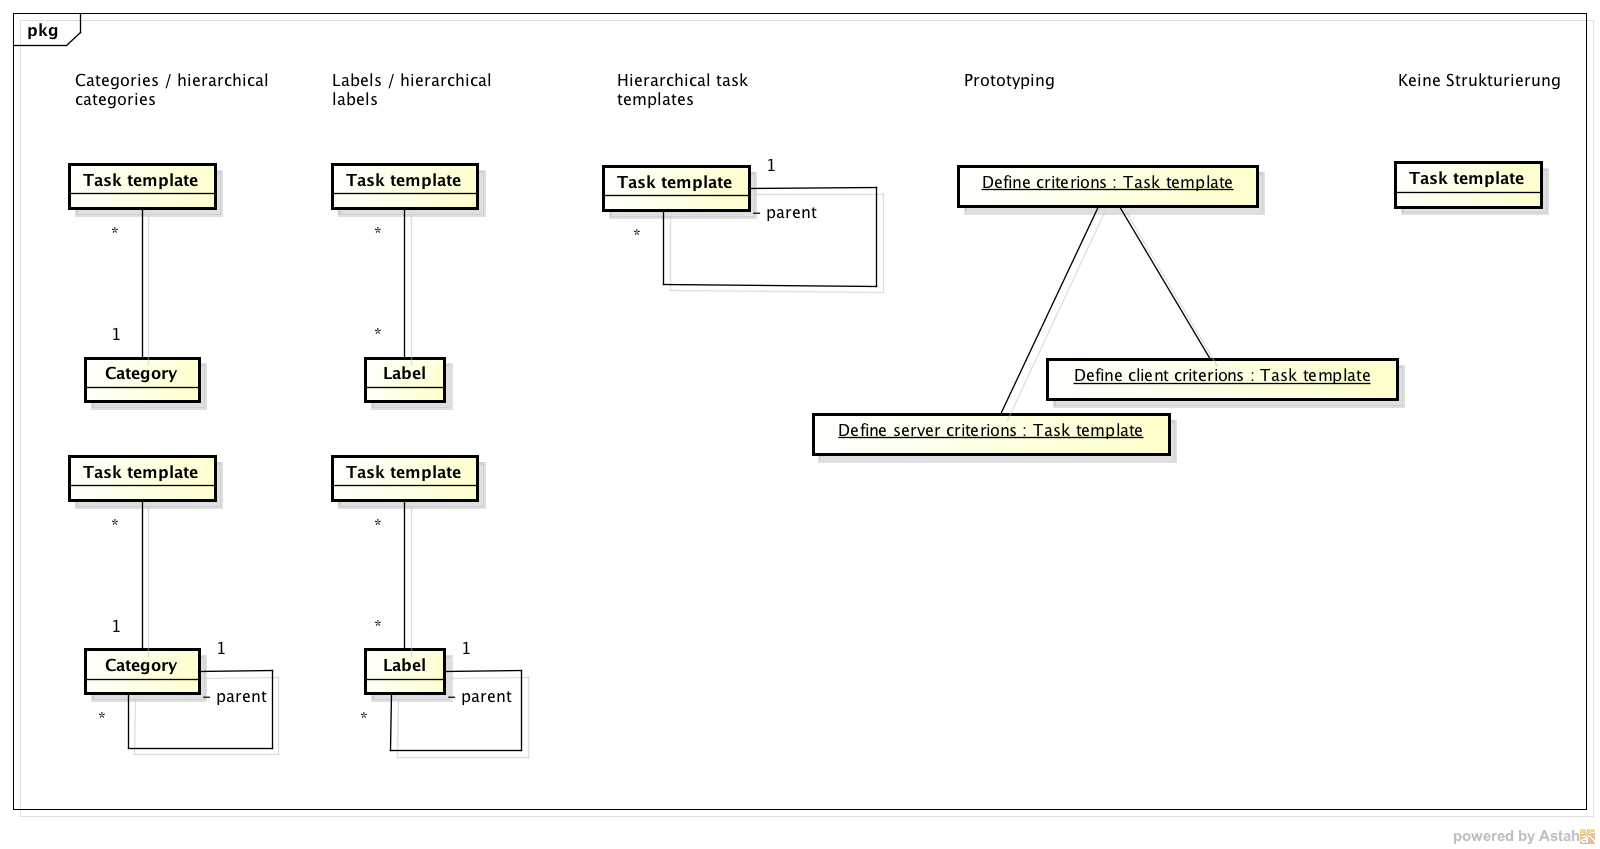
\includegraphics[width=\textwidth]{architecture/media/img/taskTemplateStructure.png}
				\centering
				\caption{Strukturierungsmöglichkeiten von Tasks}
				\label{fig:taskTemplateStructure}
			\end{figure}
			
		\decision{
			\decisionHeader{DOM-TT-STRUC}{Task-Vorlagen Strukturierung}{Architecture}{Domain}
		}{
			\decisionContent{Keine Strukturierung, allenfalls auf Wunsch des Vertreters der Anforderungsgruppe nicht hierarchische Kategorien, Smart Filters}
			{Welches Konzept soll zur Strukturierung von Task-Vorlagen eingesetzt werden?}
			{}{Benutzer sollen einfach und schnell erstellte Task-Vorlagen wieder finden.}
			{
				\begin{description}
					\item[Keine Strukturierung] \
						\begin{description}
							\item[Vorteile] Einfach zu implementieren, einfach verständlich für den Benutzer
							\item[Nachteile] Bei vielen Task-Vorlagen unübersichtlich, führt zu doppelten Task-Vorlagen da existierende nicht gefunden werden. 
						\end{description}
						
					\item[Labels/Hierarchische Labels] \
						Versehen der Elemente mit einem oder mehreren Labels. Benutzer können nach Labels suchen oder Filtern, um Vorlagen anzuzeigen.	
						\begin{description}
							\item[Vorteile] Einfach verständlich für den Benutzer
							\item[Nachteile] Benutzer könnten zu Faul sein, 
								Labels anzulegen und zuzuordnen da es aufwändiger ist als Kategorisieren
						\end{description}
					
					\item[Direkte Hierarchisierung der Task-Vorlagen] \
						Elemente werden direkt mit Elternelementen verknüpft und bilden einen hierarchischen Baum.	
						\begin{description}
							\item[Vorteile] Einfach zu implementieren
							\item[Nachteile] Schwer verständlich für den Benutzer,
								 da die Hierarchisierung unter Umständen nicht mit dem Workflow zusammenpasst
						\end{description}
					
					\item[Prototyping statt Strukturierung] \
						Elemente erben Funktionalität von einander, statt strukturiert zu werden.
						\begin{description}
							\item[Vorteile] Verringert die Anzahl Task-Vorlagen massiv, 
								da Eigenschaften vererbt werden können
							\item[Nachteile] Schwieriger umzusetzen, schwieriger zu verstehen für Benutzer
						\end{description}					
				\end{description}
			}
			{
				Keine Strukturierung hat für die Entwicklung sowie für den Benutzer Vorteile.
				So gibt es zu diesem Punkt kaum Entwicklungsaufwand 
				und der Benutzer findet trotzdem dank Suchfunktionen die gesuchten Task-Vorlagen.
				Ausserdem muss er keine Zeit aufwenden um die Task-Vorlagen zu strukturieren.

				Falls Vertreter der Anforderungsgruppe jedoch eine weitergehende Strukturierung wünschen, 
				empfehlen wir nicht-hierarchische Kategorien sowie Smart Filters.
				Kategorien erlauben eine Strukturierung auf einfache Weise. 

				Smart Filter sind eine Ergänzung zu den beiden Optionen und ermöglichen das schnelle Finden anhand von Eigenschaften ohne dass diese der Benutzer erfassen muss.
			}
			{}
			{}
			{}
		}
		
		
		\subsection{Verknüpfungen von Task-Vorlagen und Entscheidungs-Vorlagen}
			Wissensproduzenten können Task-Vorlagen zu Entscheidungs-Vorlagen zuordnen.
			Dabei kann und soll auch eine Task-Vorlage an verschiedene Entscheidungs-Vorlagen zugeordnet werden können.
			Ebenso können Entscheidungs-Vorlagen natürlich mehrere Task-Vorlagen zugeordnet erhalten.
			
			\subsubsection{Arten der Zuordnung}
				Task-Vorlagen können mit Entscheidungs-Vorlagen auf zwei Arten verknüpft werden:
				\begin{enumerate}
					\item Sie können dann fällig werden, wenn eine Entscheidung getroffen wurde (operativer Task).
					\item Eine Task-Vorlage dient dazu, Entscheidungen zu treffen (Entscheidungstask).
				\end{enumerate}
				Auf die Task-Vorlagen selbst hat dies keinen Einfluss, sie sind unabhängig davon. 
				Ob es sich um einen operativen Task oder einen Entscheidungstask handelt hängt nur davon ab,
				ob die Task-Vorlage mit einer Entscheidung (Node) oder einer Option einer Entscheidung (Subnode) des Entscheidungsbaumes verknüpft ist.

			\subsection{Übertragung von Task-Vorlagen in \ppt}
				Aus Task-Vorlagen werden beim Übertag in ein \ppt\ Tasks generiert.
				Task-Vorlagen sind generisch, da Änderungen auch alle verknüpften Problem Spaces betreffen sollen.
				Aus diesem Grund werden Task-Vorlagen bei der Zuordnung verknüpft und nicht kopiert.
				
				\begin{figure}[H]
					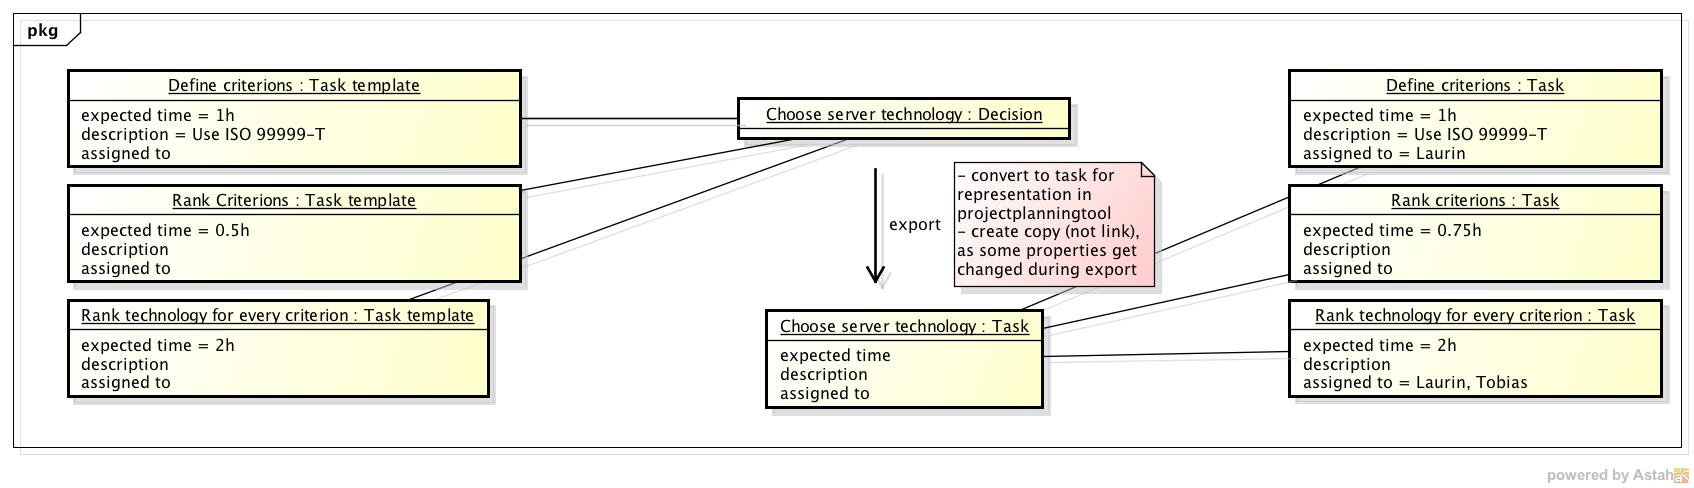
\includegraphics[width=\textwidth]{architecture/media/img/decisionTaskRelation.png}
					\centering
					\caption{Übertragen von Entscheidungen und Task-Vorlagen}
					\label{fig:DecisionTaskRelation}
				\end{figure}
				
				Beim Übertragen werden aus Task-Vorlagen (konkrete) Tasks.
				Auch Entscheidungen werden zu Tasks übertragen, da \ppt's keine Entscheidungen kennen.
				Mit Entscheidungen verknüpfte Tasks werden entsprechend zu Sub-Tasks.
				
				Benutzer wollen bei der Übertragung ins \ppt\ die von der Task-Vorlage vorgegebenen Werte möglicherweise anpassen, wie z.B. den erwarteten Aufwand für den Task.
				Daher ist es sinnvoll, die Eigenschaften der Task-Vorlagen in die (konkreten) Tasks zu kopieren, anstatt sie lediglich zu verknüpfen.
				Gleiches gilt für Entscheidungen. Würde jemand im \cdar\ diese verändern oder Löschen, so würde dies die History zerstören.
			
		
		\subsection{Tasktransmission Workflow}
			Aus Task-Vorlagen erzeugte Tasks müssen zur Übertragung in ein Projektmanagementtool
			Tool spezifisch umgewandelt werden. Dazu werden "`Processors"' eingesetzt.
			Processors stellen kleine Funktionalitäten dar, die Daten umwandeln, wie z.B. "`Date processors"', die Kalenderdaten umwandeln, "`Issue type processors"', die Issuetypes konvertieren, "`User processors"', die Relationen zu Benutzern so umwandeln, das das Projektplanungstool den User korrekt verknüpfen kann oder "`Conditional processors"' und "`Option processors"', die Bedingungen verarbeiten.
			Ebenfalls denkbar ist ein Processor, der Felder aggregieren kann und damit z.B. nicht gemappte Felder in die Beschreibung überführen kann.
			
			\begin{figure}[H]
				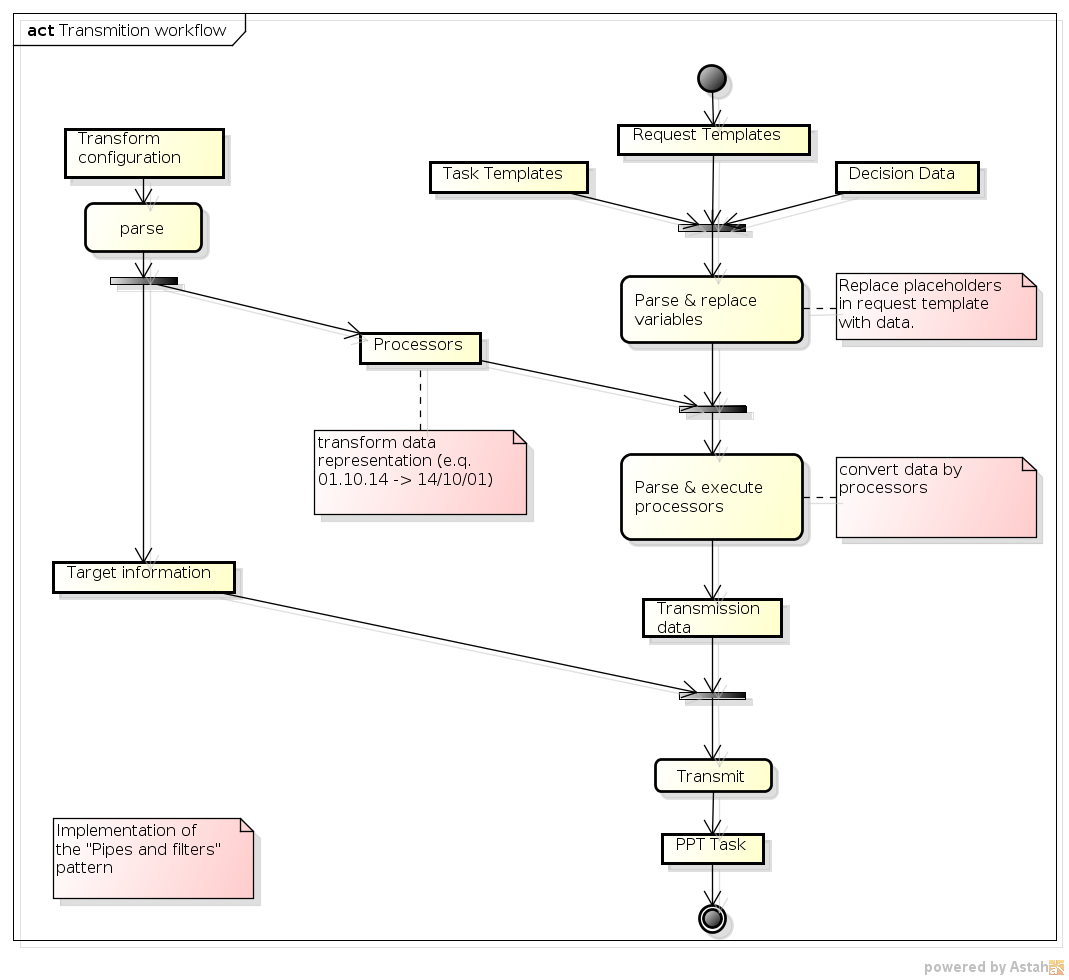
\includegraphics[width=\textwidth]{architecture/media/img/transmissionWorkflow.png}
				\centering
				\caption{Übertragen von Tasks}
				\label{fig:transmissionWorkflow}
			\end{figure}
			Dem Transmissionworkflow liegt das "`Pipes and filters"' Pattern zugrunde
			 \cite{hope_enterprise_2003}, welches eine Verarbeitungs- und Filterkette definiert.
			
			Der komplette Tasktransmission Workflow soll auf dem Client durchgeführt werden und nicht auf dem Server. Grund dafür sind einerseits die Problematik, 
			das sich der \eeppi\ Server in einer Zone befinden kann, 
			die ihm keinen direkten Zugriff auf den \ppt-Server erlaubt,
			andererseits schränkt die Wahl der Servertechnologie die Möglichkeiten für dynamische Processors ein, während die Client Technologie dies ermöglicht.
			
			Im Laufe der Erarbeitung dieses Workflows wurde auch darüber nachgedacht, 
			wie Eigenschaften verarbeitet werden sollen, die nicht gemappt wurden. 
			Ursprünglich wurde entschieden, diese in Listenform in die Beschreibung des Tasks
			überzuführen. 
			Die Entscheidung für ein sehr flexibles Mapping führte dazu, 
			das dieser Anwendungsfall überflüssig wurde, 
			weil der Administrator dazu selbst einen Processor definieren kann.
			Womit die Entscheidung darüber bei ihm bleibt und nicht von uns vorgegeben wird.
			Zudem müsste in jedem Fall bekannt sein, 
			bei welchem Feld es sich um das Beschreibungsfeld handelt, 
			was nicht gegeben ist, wenn der Administrator vergisst, dies zu konfigurieren.
		
		
		\subsection{Mapping Method}
		\decision{
			\decisionHeader{DOM-TT-MM}{Mapping method}{Architecture}{Domain}
		}{
			\decisionContent{Konfiguration/Block in Form von Templates mit Plathaltern}
			{Wie sollen Mappingkonfigurationen erstellt werden?}
			{}
			{Von der Mapping Method hängt die Architektur des Mappings und die Schnittstellen der Processors und Filters ab.}
			{
				\begin{description}					
					\item[Hierarchische/Element basierte Konfiguration] \
					Das Mapping wird durch das Anlegen von verknüpften Elementen erzeugt.
					\begin{description}
						\item[Vorteile] Gegebene Validierung durch die Struktur, kein Parser notwendig
						\item[Nachteile] Aufwändiger umzusetzen, insbesondere das UI, weniger flexibel
					\end{description}
				\end{description}
			}
			{Eine Textblock/Template-basierte Konfiguration erhöht zwar die Fehlermöglichkeiten für den Administrator,
			ermöglicht diesem jedoch grössere Flexibilität und damit ein Abdecken einer grösseren Bandbreite an Projektplanungstools.}
			{Der Administrator kann mit Templates und Platzhaltern umgehen oder es Lernen}
			{Das Mapping benötigt kein eigenes Datenmodell in Form von verknüpften Objekten. 
			Es kann als einfache Text-Elemente an ein Projekt angeknüpft werden.}
			{}
		}
		
		Der Ablauf für einen Administrator sieht entsprechend wie folgt aus:
		\begin{enumerate}
			\item Projektplanungstool definieren
			\item Taskeigenschaften erstellen
			\item Mapping Taskeigenschaften -> Projektplanungstool erstellen
		\end{enumerate}
		
		
		\subsection{EEPPI Domain}
			
				
		
		\subsection{Communication}